% Generated by libra_sparging/make_closure_diagram.py -- do not edit by hand.
% Requires: \usetikzlibrary{positioning, fit, backgrounds, arrows.meta}
\begin{figure}[htbp]
\centering
\resizebox{\linewidth}{!}{%
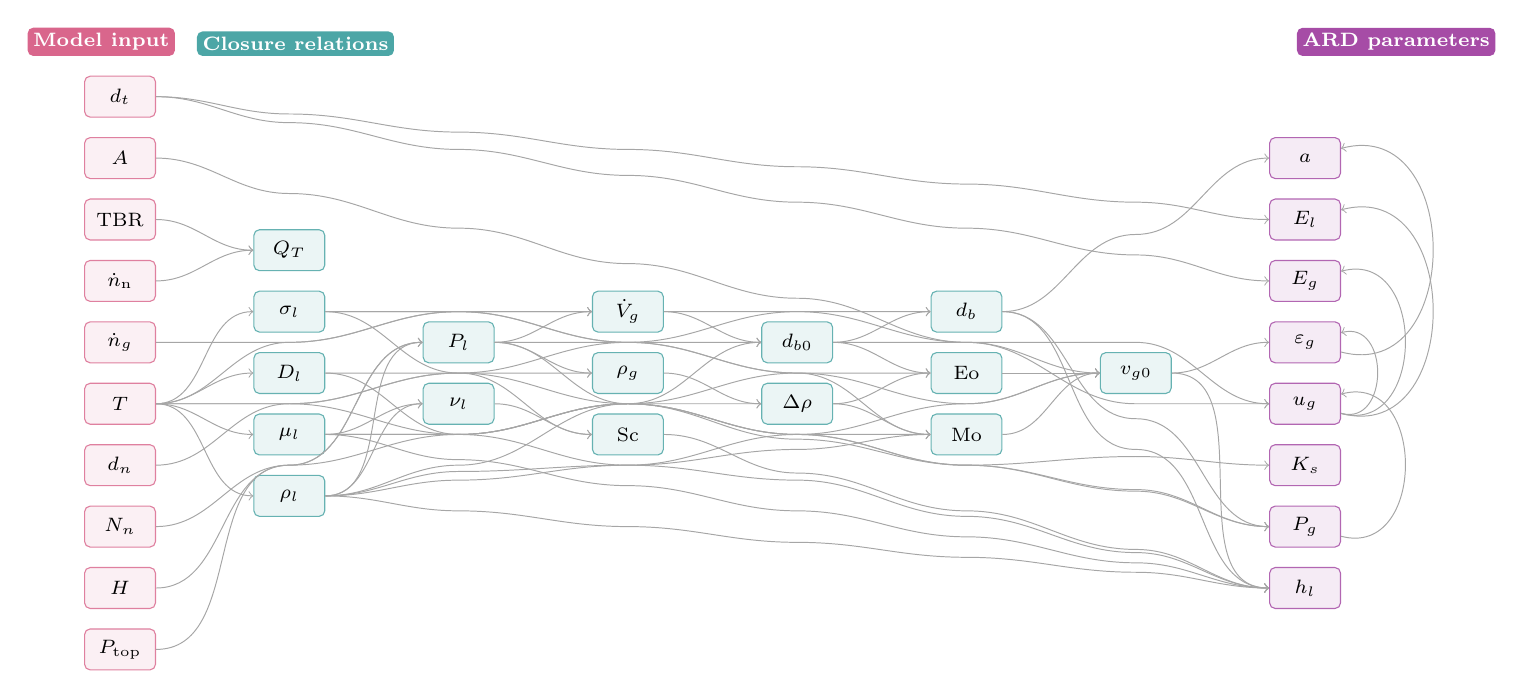
\begin{tikzpicture}[
  font=\scriptsize,
  boxbase/.style={draw=black!55, rounded corners=2pt, fill=white,
                  minimum height=5.2mm, minimum width=9mm, inner sep=1.5pt},
  boxin/.style={boxbase, fill=purple!6, draw=purple!50},
  boxclos/.style={boxbase, fill=teal!8, draw=teal!60},
  boxard/.style={boxbase, fill=violet!8, draw=violet!60},
  arr/.style={->, draw=black!35, line width=0.35pt},
  tag/.style={anchor=south west, fill=#1, text=white,
              font=\scriptsize\bfseries, inner sep=2pt, rounded corners=2pt},
]

% ---- column 0 ----
\node[boxin] (P_top) at (0.00, 0.00) {$P_\mathrm{top}$};
\node[boxin] (height) at (0.00, 0.78) {$H$};
\node[boxin] (nb_nozzle) at (0.00, 1.56) {$N_n$};
\node[boxin] (nozzle_diameter) at (0.00, 2.34) {$d_n$};
\node[boxin] (temperature) at (0.00, 3.12) {$T$};
\node[boxin] (ndot_g0) at (0.00, 3.90) {$\dot n_g$};
\node[boxin] (n_gen_rate) at (0.00, 4.68) {$\dot n_\mathrm{n}$};
\node[boxin] (tbr) at (0.00, 5.46) {TBR};
\node[boxin] (area) at (0.00, 6.24) {$A$};
\node[boxin] (tank_diameter) at (0.00, 7.02) {$d_t$};

% ---- column 1 ----
\node[boxclos] (rho_l) at (2.15, 1.95) {$\rho_l$};
\node[boxclos] (mu_l) at (2.15, 2.73) {$\mu_l$};
\node[boxclos] (D_l) at (2.15, 3.51) {$D_l$};
\node[boxclos] (sigma_l) at (2.15, 4.29) {$\sigma_l$};
\node[boxclos] (Q_T) at (2.15, 5.07) {$Q_T$};

% ---- column 2 ----
\node[boxclos] (nu_l) at (4.30, 3.12) {$\nu_l$};
\node[boxclos] (P_l_0) at (4.30, 3.90) {$P_l$};

% ---- column 3 ----
\node[boxclos] (Sc) at (6.45, 2.73) {Sc};
\node[boxclos] (rho_g) at (6.45, 3.51) {$\rho_g$};
\node[boxclos] (Vdot_g0) at (6.45, 4.29) {$\dot V_g$};

% ---- column 4 ----
\node[boxclos] (drho) at (8.60, 3.12) {$\Delta\rho$};
\node[boxclos] (d_b0) at (8.60, 3.90) {$d_{b0}$};

% ---- column 5 ----
\node[boxclos] (Mo) at (10.75, 2.73) {Mo};
\node[boxclos] (Eo) at (10.75, 3.51) {Eo};
\node[boxclos] (d_b_0) at (10.75, 4.29) {$d_b$};

% ---- column 6 ----
\node[boxclos] (v_g0) at (12.90, 3.51) {$v_{g0}$};

% ---- column 7 ----
\node[boxard] (h_l_0) at (15.05, 0.78) {$h_l$};
\node[boxard] (P_g_0) at (15.05, 1.56) {$P_g$};
\node[boxard] (K_s) at (15.05, 2.34) {$K_s$};
\node[boxard] (u_g_0) at (15.05, 3.12) {$u_g$};
\node[boxard] (eps_g_0) at (15.05, 3.90) {$\varepsilon_g$};
\node[boxard] (E_g) at (15.05, 4.68) {$E_g$};
\node[boxard] (E_l) at (15.05, 5.46) {$E_l$};
\node[boxard] (a_0) at (15.05, 6.24) {$a$};

% ---- routing waypoints for the long dependencies ----
\coordinate (dummy_height_P_l_0_1) at (2.15, 2.34);
\coordinate (dummy_area_u_g_0_1) at (2.15, 5.79);
\coordinate (dummy_area_u_g_0_2) at (4.30, 5.35);
\coordinate (dummy_area_u_g_0_3) at (6.45, 4.90);
\coordinate (dummy_area_u_g_0_4) at (8.60, 4.46);
\coordinate (dummy_area_u_g_0_5) at (10.75, 3.90);
\coordinate (dummy_area_u_g_0_6) at (12.90, 3.90);
\coordinate (dummy_temperature_K_s_1) at (2.15, 3.12);
\coordinate (dummy_temperature_K_s_2) at (4.30, 2.73);
\coordinate (dummy_temperature_K_s_3) at (6.45, 3.12);
\coordinate (dummy_temperature_K_s_4) at (8.60, 2.67);
\coordinate (dummy_temperature_K_s_5) at (10.75, 2.34);
\coordinate (dummy_temperature_K_s_6) at (12.90, 2.45);
\coordinate (dummy_temperature_Vdot_g0_1) at (2.15, 3.90);
\coordinate (dummy_temperature_Vdot_g0_2) at (4.30, 4.29);
\coordinate (dummy_temperature_rho_g_1) at (2.15, 3.12);
\coordinate (dummy_temperature_rho_g_2) at (4.30, 3.51);
\coordinate (dummy_rho_l_v_g0_2) at (4.30, 2.26);
\coordinate (dummy_rho_l_v_g0_3) at (6.45, 2.34);
\coordinate (dummy_rho_l_v_g0_4) at (8.60, 2.73);
\coordinate (dummy_rho_l_v_g0_5) at (10.75, 3.12);
\coordinate (dummy_rho_l_drho_2) at (4.30, 2.34);
\coordinate (dummy_rho_l_drho_3) at (6.45, 3.12);
\coordinate (dummy_rho_l_Mo_2) at (4.30, 2.15);
\coordinate (dummy_rho_l_Mo_3) at (6.45, 2.34);
\coordinate (dummy_rho_l_Mo_4) at (8.60, 2.54);
\coordinate (dummy_rho_l_h_l_0_2) at (4.30, 1.76);
\coordinate (dummy_rho_l_h_l_0_3) at (6.45, 1.56);
\coordinate (dummy_rho_l_h_l_0_4) at (8.60, 1.36);
\coordinate (dummy_rho_l_h_l_0_5) at (10.75, 1.17);
\coordinate (dummy_rho_l_h_l_0_6) at (12.90, 0.98);
\coordinate (dummy_tank_diameter_E_g_1) at (2.15, 6.69);
\coordinate (dummy_tank_diameter_E_g_2) at (4.30, 6.35);
\coordinate (dummy_tank_diameter_E_g_3) at (6.45, 6.02);
\coordinate (dummy_tank_diameter_E_g_4) at (8.60, 5.68);
\coordinate (dummy_tank_diameter_E_g_5) at (10.75, 5.35);
\coordinate (dummy_tank_diameter_E_g_6) at (12.90, 5.01);
\coordinate (dummy_tank_diameter_E_l_1) at (2.15, 6.80);
\coordinate (dummy_tank_diameter_E_l_2) at (4.30, 6.57);
\coordinate (dummy_tank_diameter_E_l_3) at (6.45, 6.35);
\coordinate (dummy_tank_diameter_E_l_4) at (8.60, 6.13);
\coordinate (dummy_tank_diameter_E_l_5) at (10.75, 5.91);
\coordinate (dummy_tank_diameter_E_l_6) at (12.90, 5.68);
\coordinate (dummy_Vdot_g0_u_g_0_4) at (8.60, 4.29);
\coordinate (dummy_Vdot_g0_u_g_0_5) at (10.75, 3.90);
\coordinate (dummy_Vdot_g0_u_g_0_6) at (12.90, 3.12);
\coordinate (dummy_ndot_g0_Vdot_g0_1) at (2.15, 3.90);
\coordinate (dummy_ndot_g0_Vdot_g0_2) at (4.30, 4.29);
\coordinate (dummy_P_l_0_P_g_0_3) at (6.45, 3.12);
\coordinate (dummy_P_l_0_P_g_0_4) at (8.60, 2.73);
\coordinate (dummy_P_l_0_P_g_0_5) at (10.75, 2.34);
\coordinate (dummy_P_l_0_P_g_0_6) at (12.90, 2.03);
\coordinate (dummy_P_l_0_d_b_0_3) at (6.45, 3.90);
\coordinate (dummy_P_l_0_d_b_0_4) at (8.60, 4.29);
\coordinate (dummy_P_top_P_l_0_1) at (2.15, 2.34);
\coordinate (dummy_d_b_0_P_g_0_6) at (12.90, 2.93);
\coordinate (dummy_d_b_0_a_0_6) at (12.90, 5.27);
\coordinate (dummy_d_b_0_h_l_0_6) at (12.90, 2.54);
\coordinate (dummy_sigma_l_P_g_0_2) at (4.30, 3.51);
\coordinate (dummy_sigma_l_P_g_0_3) at (6.45, 3.12);
\coordinate (dummy_sigma_l_P_g_0_4) at (8.60, 2.73);
\coordinate (dummy_sigma_l_P_g_0_5) at (10.75, 2.34);
\coordinate (dummy_sigma_l_P_g_0_6) at (12.90, 2.01);
\coordinate (dummy_sigma_l_Eo_2) at (4.30, 4.29);
\coordinate (dummy_sigma_l_Eo_3) at (6.45, 3.90);
\coordinate (dummy_sigma_l_Eo_4) at (8.60, 3.51);
\coordinate (dummy_sigma_l_Mo_2) at (4.30, 4.29);
\coordinate (dummy_sigma_l_Mo_3) at (6.45, 3.90);
\coordinate (dummy_sigma_l_Mo_4) at (8.60, 3.51);
\coordinate (dummy_d_b0_v_g0_5) at (10.75, 3.90);
\coordinate (dummy_nozzle_diameter_d_b0_1) at (2.15, 3.12);
\coordinate (dummy_nozzle_diameter_d_b0_2) at (4.30, 3.51);
\coordinate (dummy_nozzle_diameter_d_b0_3) at (6.45, 3.90);
\coordinate (dummy_nb_nozzle_d_b0_1) at (2.15, 2.34);
\coordinate (dummy_nb_nozzle_d_b0_2) at (4.30, 2.73);
\coordinate (dummy_nb_nozzle_d_b0_3) at (6.45, 3.12);
\coordinate (dummy_mu_l_v_g0_2) at (4.30, 2.73);
\coordinate (dummy_mu_l_v_g0_3) at (6.45, 3.12);
\coordinate (dummy_mu_l_v_g0_4) at (8.60, 3.51);
\coordinate (dummy_mu_l_v_g0_5) at (10.75, 3.12);
\coordinate (dummy_mu_l_Mo_2) at (4.30, 2.73);
\coordinate (dummy_mu_l_Mo_3) at (6.45, 3.12);
\coordinate (dummy_mu_l_Mo_4) at (8.60, 2.73);
\coordinate (dummy_mu_l_h_l_0_2) at (4.30, 2.41);
\coordinate (dummy_mu_l_h_l_0_3) at (6.45, 2.08);
\coordinate (dummy_mu_l_h_l_0_4) at (8.60, 1.76);
\coordinate (dummy_mu_l_h_l_0_5) at (10.75, 1.43);
\coordinate (dummy_mu_l_h_l_0_6) at (12.90, 1.10);
\coordinate (dummy_Sc_h_l_0_4) at (8.60, 2.24);
\coordinate (dummy_Sc_h_l_0_5) at (10.75, 1.76);
\coordinate (dummy_Sc_h_l_0_6) at (12.90, 1.27);
\coordinate (dummy_D_l_h_l_0_2) at (4.30, 2.73);
\coordinate (dummy_D_l_h_l_0_3) at (6.45, 2.34);
\coordinate (dummy_D_l_h_l_0_4) at (8.60, 2.15);
\coordinate (dummy_D_l_h_l_0_5) at (10.75, 1.69);
\coordinate (dummy_D_l_h_l_0_6) at (12.90, 1.23);
\coordinate (dummy_D_l_Sc_2) at (4.30, 3.51);

% ---- dependencies ----
\draw[arr] (D_l) to[out=0,in=180] (dummy_D_l_Sc_2) to[out=0,in=180] (Sc);
\draw[arr] (D_l) to[out=0,in=180] (dummy_D_l_h_l_0_2) to[out=0,in=180] (dummy_D_l_h_l_0_3) to[out=0,in=180] (dummy_D_l_h_l_0_4) to[out=0,in=180] (dummy_D_l_h_l_0_5) to[out=0,in=180] (dummy_D_l_h_l_0_6) to[out=0,in=180] (h_l_0);
\draw[arr] (P_l_0) to[out=0,in=180] (dummy_P_l_0_P_g_0_3) to[out=0,in=180] (dummy_P_l_0_P_g_0_4) to[out=0,in=180] (dummy_P_l_0_P_g_0_5) to[out=0,in=180] (dummy_P_l_0_P_g_0_6) to[out=0,in=180] (P_g_0);
\draw[arr] (P_l_0) to[out=0,in=180] (dummy_P_l_0_d_b_0_3) to[out=0,in=180] (dummy_P_l_0_d_b_0_4) to[out=0,in=180] (d_b_0);
\draw[arr] (P_top) to[out=0,in=180] (dummy_P_top_P_l_0_1) to[out=0,in=180] (P_l_0);
\draw[arr] (Sc) to[out=0,in=180] (dummy_Sc_h_l_0_4) to[out=0,in=180] (dummy_Sc_h_l_0_5) to[out=0,in=180] (dummy_Sc_h_l_0_6) to[out=0,in=180] (h_l_0);
\draw[arr] (Vdot_g0) to[out=0,in=180] (dummy_Vdot_g0_u_g_0_4) to[out=0,in=180] (dummy_Vdot_g0_u_g_0_5) to[out=0,in=180] (dummy_Vdot_g0_u_g_0_6) to[out=0,in=180] (u_g_0);
\draw[arr] (area) to[out=0,in=180] (dummy_area_u_g_0_1) to[out=0,in=180] (dummy_area_u_g_0_2) to[out=0,in=180] (dummy_area_u_g_0_3) to[out=0,in=180] (dummy_area_u_g_0_4) to[out=0,in=180] (dummy_area_u_g_0_5) to[out=0,in=180] (dummy_area_u_g_0_6) to[out=0,in=180] (u_g_0);
\draw[arr] (d_b0) to[out=0,in=180] (dummy_d_b0_v_g0_5) to[out=0,in=180] (v_g0);
\draw[arr] (d_b_0) to[out=0,in=180] (dummy_d_b_0_P_g_0_6) to[out=0,in=180] (P_g_0);
\draw[arr] (d_b_0) to[out=0,in=180] (dummy_d_b_0_a_0_6) to[out=0,in=180] (a_0);
\draw[arr] (d_b_0) to[out=0,in=180] (dummy_d_b_0_h_l_0_6) to[out=0,in=180] (h_l_0);
\draw[arr] (height) to[out=0,in=180] (dummy_height_P_l_0_1) to[out=0,in=180] (P_l_0);
\draw[arr] (mu_l) to[out=0,in=180] (dummy_mu_l_Mo_2) to[out=0,in=180] (dummy_mu_l_Mo_3) to[out=0,in=180] (dummy_mu_l_Mo_4) to[out=0,in=180] (Mo);
\draw[arr] (mu_l) to[out=0,in=180] (dummy_mu_l_h_l_0_2) to[out=0,in=180] (dummy_mu_l_h_l_0_3) to[out=0,in=180] (dummy_mu_l_h_l_0_4) to[out=0,in=180] (dummy_mu_l_h_l_0_5) to[out=0,in=180] (dummy_mu_l_h_l_0_6) to[out=0,in=180] (h_l_0);
\draw[arr] (mu_l) to[out=0,in=180] (dummy_mu_l_v_g0_2) to[out=0,in=180] (dummy_mu_l_v_g0_3) to[out=0,in=180] (dummy_mu_l_v_g0_4) to[out=0,in=180] (dummy_mu_l_v_g0_5) to[out=0,in=180] (v_g0);
\draw[arr] (nb_nozzle) to[out=0,in=180] (dummy_nb_nozzle_d_b0_1) to[out=0,in=180] (dummy_nb_nozzle_d_b0_2) to[out=0,in=180] (dummy_nb_nozzle_d_b0_3) to[out=0,in=180] (d_b0);
\draw[arr] (ndot_g0) to[out=0,in=180] (dummy_ndot_g0_Vdot_g0_1) to[out=0,in=180] (dummy_ndot_g0_Vdot_g0_2) to[out=0,in=180] (Vdot_g0);
\draw[arr] (nozzle_diameter) to[out=0,in=180] (dummy_nozzle_diameter_d_b0_1) to[out=0,in=180] (dummy_nozzle_diameter_d_b0_2) to[out=0,in=180] (dummy_nozzle_diameter_d_b0_3) to[out=0,in=180] (d_b0);
\draw[arr] (rho_l) to[out=0,in=180] (dummy_rho_l_Mo_2) to[out=0,in=180] (dummy_rho_l_Mo_3) to[out=0,in=180] (dummy_rho_l_Mo_4) to[out=0,in=180] (Mo);
\draw[arr] (rho_l) to[out=0,in=180] (dummy_rho_l_drho_2) to[out=0,in=180] (dummy_rho_l_drho_3) to[out=0,in=180] (drho);
\draw[arr] (rho_l) to[out=0,in=180] (dummy_rho_l_h_l_0_2) to[out=0,in=180] (dummy_rho_l_h_l_0_3) to[out=0,in=180] (dummy_rho_l_h_l_0_4) to[out=0,in=180] (dummy_rho_l_h_l_0_5) to[out=0,in=180] (dummy_rho_l_h_l_0_6) to[out=0,in=180] (h_l_0);
\draw[arr] (rho_l) to[out=0,in=180] (dummy_rho_l_v_g0_2) to[out=0,in=180] (dummy_rho_l_v_g0_3) to[out=0,in=180] (dummy_rho_l_v_g0_4) to[out=0,in=180] (dummy_rho_l_v_g0_5) to[out=0,in=180] (v_g0);
\draw[arr] (sigma_l) to[out=0,in=180] (dummy_sigma_l_Eo_2) to[out=0,in=180] (dummy_sigma_l_Eo_3) to[out=0,in=180] (dummy_sigma_l_Eo_4) to[out=0,in=180] (Eo);
\draw[arr] (sigma_l) to[out=0,in=180] (dummy_sigma_l_Mo_2) to[out=0,in=180] (dummy_sigma_l_Mo_3) to[out=0,in=180] (dummy_sigma_l_Mo_4) to[out=0,in=180] (Mo);
\draw[arr] (sigma_l) to[out=0,in=180] (dummy_sigma_l_P_g_0_2) to[out=0,in=180] (dummy_sigma_l_P_g_0_3) to[out=0,in=180] (dummy_sigma_l_P_g_0_4) to[out=0,in=180] (dummy_sigma_l_P_g_0_5) to[out=0,in=180] (dummy_sigma_l_P_g_0_6) to[out=0,in=180] (P_g_0);
\draw[arr] (tank_diameter) to[out=0,in=180] (dummy_tank_diameter_E_g_1) to[out=0,in=180] (dummy_tank_diameter_E_g_2) to[out=0,in=180] (dummy_tank_diameter_E_g_3) to[out=0,in=180] (dummy_tank_diameter_E_g_4) to[out=0,in=180] (dummy_tank_diameter_E_g_5) to[out=0,in=180] (dummy_tank_diameter_E_g_6) to[out=0,in=180] (E_g);
\draw[arr] (tank_diameter) to[out=0,in=180] (dummy_tank_diameter_E_l_1) to[out=0,in=180] (dummy_tank_diameter_E_l_2) to[out=0,in=180] (dummy_tank_diameter_E_l_3) to[out=0,in=180] (dummy_tank_diameter_E_l_4) to[out=0,in=180] (dummy_tank_diameter_E_l_5) to[out=0,in=180] (dummy_tank_diameter_E_l_6) to[out=0,in=180] (E_l);
\draw[arr] (temperature) to[out=0,in=180] (dummy_temperature_K_s_1) to[out=0,in=180] (dummy_temperature_K_s_2) to[out=0,in=180] (dummy_temperature_K_s_3) to[out=0,in=180] (dummy_temperature_K_s_4) to[out=0,in=180] (dummy_temperature_K_s_5) to[out=0,in=180] (dummy_temperature_K_s_6) to[out=0,in=180] (K_s);
\draw[arr] (temperature) to[out=0,in=180] (dummy_temperature_Vdot_g0_1) to[out=0,in=180] (dummy_temperature_Vdot_g0_2) to[out=0,in=180] (Vdot_g0);
\draw[arr] (temperature) to[out=0,in=180] (dummy_temperature_rho_g_1) to[out=0,in=180] (dummy_temperature_rho_g_2) to[out=0,in=180] (rho_g);
\draw[arr] (Eo) to[out=0,in=180] (v_g0);
\draw[arr] (Mo) to[out=0,in=180] (v_g0);
\draw[arr] (P_g_0) to[out=-15,in=15,looseness=1.6] (u_g_0);
\draw[arr] (P_l_0) to[out=0,in=180] (Vdot_g0);
\draw[arr] (P_l_0) to[out=0,in=180] (rho_g);
\draw[arr] (Vdot_g0) to[out=0,in=180] (d_b0);
\draw[arr] (d_b0) to[out=0,in=180] (Eo);
\draw[arr] (d_b0) to[out=0,in=180] (d_b_0);
\draw[arr] (drho) to[out=0,in=180] (Eo);
\draw[arr] (drho) to[out=0,in=180] (Mo);
\draw[arr] (eps_g_0) to[out=-15,in=15,looseness=1.6] (a_0);
\draw[arr] (mu_l) to[out=0,in=180] (nu_l);
\draw[arr] (n_gen_rate) to[out=0,in=180] (Q_T);
\draw[arr] (nu_l) to[out=0,in=180] (Sc);
\draw[arr] (rho_g) to[out=0,in=180] (drho);
\draw[arr] (rho_l) to[out=0,in=180] (P_l_0);
\draw[arr] (rho_l) to[out=0,in=180] (nu_l);
\draw[arr] (tbr) to[out=0,in=180] (Q_T);
\draw[arr] (temperature) to[out=0,in=180] (D_l);
\draw[arr] (temperature) to[out=0,in=180] (mu_l);
\draw[arr] (temperature) to[out=0,in=180] (rho_l);
\draw[arr] (temperature) to[out=0,in=180] (sigma_l);
\draw[arr] (u_g_0) to[out=-15,in=15,looseness=1.6] (E_g);
\draw[arr] (u_g_0) to[out=-15,in=15,looseness=1.6] (E_l);
\draw[arr] (u_g_0) to[out=-15,in=15,looseness=1.6] (eps_g_0);
\draw[arr] (v_g0) to[out=0,in=180] (eps_g_0);
\draw[arr] (v_g0) to[out=0,in=180] (h_l_0);

% ---- stage labels, matching diag_model_overview ----
\node[tag=purple!60] at (-1.18, 7.53) {Model input};
\node[tag=teal!70] at (0.97, 7.53) {Closure relations};
\node[tag=violet!70] at (14.94, 7.53) {ARD parameters};
\end{tikzpicture}%
}
\caption{Dependency network of the closure relations, resolved for the LIBRA Pi case. Each column holds the parameters that sit at the same depth in the dependency graph, so the flow runs from the model inputs on the left to the parameters the 1D ARD equations consume on the right. This is the \textbf{closure relations} stage of \cref{fig:model_overview} seen from close up.}
\label{fig:closure_graph}
\end{figure}
